\documentclass[man,floatsintext]{apa6}
\usepackage[nodoi]{apacite}
\usepackage{graphicx}
\usepackage[american]{babel}
\usepackage{amsmath}
\usepackage{enumitem}
\usepackage[section]{placeins}
\usepackage{caption}
\usepackage{subcaption}

\title{Adults and preschoolers flexibly adapt to noisy linguistic input}
\author{Daniel Yurovsky, Sarah Case, and Michael C. Frank}
\affiliation{Stanford University}
\shorttitle{Noisy Kids}
\leftheader{Yurovsky \& Frank}


\abstract{
}

\keywords{Language processing, noisy channel, cognitive development}

\authornote{Please address correspondence to: 

\vspace{12 pt}
Daniel Yurovsky

Jordan Hall (Building 420)

Stanford University

450 Serra Mall

Stanford, CA 94305

\vspace{12 pt}
Email: yurovsky@stanford.edu 

\vspace{24 pt}

Word Count: 
}

\begin{document}
\maketitle

Imagine Bob hears Alice say ``I had carrots and bees for dinner.'' Perhaps she visited an exotic restaurant, and he should follow up and ask how they tasted. Or perhaps he misheard her, or she misspoke (she actually had peas). Interpreting her utterance requires integrating perceptual information about what he heard with his expectations: about both what words usually go with ``carrots'' and ``dinner'' and also what foods people usually eat. Modern statistical language processing systems operate using a body of theory based on this idea---that language is a \emph{noisy channel}, and that Bob can correct for perceptual errors using linguistic expectations about what Alice was likely trying to say \cite{jelinek1976, shannon1948}. 

Noisy channel principles provide a powerful framework for explaining how the human language processing system operates in complex and uncertain real-time communicative situations \cite{clayards2008, levy2008, jaeger2010, kleinschmidt2015}. On this view of human language, comprehenders integrate prior expectations with perceptual data; and they do so probabilistically, weighting each according to its reliability \cite{ernst2002, jacobs1999}. In one demonstration of this kind of integration, \citeA{gibson2013} presented participants with semantically implausible sentences (e.g., ``The mother gave the candle the daughter''), which could have been produced by small typographical errors in otherwise much more plausible sentences (e.g., the omission of the word ``to''). Adult comprehenders were able to correct these errors, and critically corrected them at higher rates when they had reason to believe that the communicative channel was noisy (and hence the perceptual signal was unreliable). Conversely, they corrected these errors at lower rates when they believed they were in a ``silly'' context where many of the sentences they read were similarly implausible. Together, these resutls suggested a flexible weighting on the perceptual signal---channel noise---and prior expectations---speaker plausibility. 

Do children also do the same kind of flexible, expectation-based language processing? Prior research on this topic is mixed. On one hand, infants and toddlers already make use of speakers' social and pragmatic cues to reference \cite{clark2009, carpenter1998}. And preschoolers show evidence of encoding stable features like the reliability of individual speakers \cite{koenig2004, harris2012}. On the other hand, the children at the same ages sometimes show striking deficits in pragmatic reasoning about speakers' intentions \cite{noveck2001} and have trouble revising their first interpretation of syntactic ambiguities \cite{trueswell1999}. Our current experiments thus attempt to test whether young children flexibly integrate expectations about speakers with the noise in a communicative channel. 

We created a paradigm that allowed us to manipulate both expectations about a speaker's plausibility and perceptual noise. We introduced four- and five-year-old children (and adults) to either a plausible or implausible speaker, who initially uttered unambiguous sentences like ``my cat has three little [kittens/hammers]'' (Figure \ref{fig:exposure}). We then asked participants to resolve the intended meaning for ambiguous sentences such as the ``bees/peas'' example above, which could either be the product of a mishearing or phonological error, or could convey implausible content (Figure \ref{fig:test}). We predicted that, if children are able to integrate speaker expectations and channel noise, then their interpretations should be a product of both of these. In Experiment 1, we provide a first test of this hypothesis by manipulating speaker plausibility. In Experiment 2, we replicate the findings of Experiment 1 and cross these with a manipulation of channel noise. The results of these two experiments support the idea that children, as well as adults, show evidence of flexibly trading off between information sources in language comprehension.

\begin{figure}[tb]
     \centering
        \begin{subfigure}[b]{.4 \textwidth}
            \caption{\label{fig:exposure}}
            
\includegraphics[width=\textwidth]{figures/exposure.pdf}
        \end{subfigure}\\
        \vspace{12 pt}
        \begin{subfigure}[b]{.4 \textwidth}
           \caption{\label{fig:test}}
           
\includegraphics[width=\textwidth]{figures/testing.pdf}
        \end{subfigure}
    \caption{Example Exposure and Test trials. On Exposure trials, the two pictures and their corresponding referring expressions were highly distinct (e.g. ``my cat has three little [kittens/hammers].'' In contrast, the two pictures on Test trials could be referred to by expressions that contained a single phonological error (e.g. I had carrots and [bees/peas] for dinner.'' For participants in the Implausible condition, the speaker referred to the implausible referent (e.g. ``hammers'') on all Exposure trials. For participants in the Plausible condition, the speaker referred to to the plausible referent on all Exposure trials (e.g. ``kittens''). On test trials, the speaker always referred to the implausible referent (``bees'').}
   \label{fig:stimuli}
\end{figure}


\section{Experiment 1}

\subsection{Method}
\subsubsection{Participants}

Adult participants for Experiment 1 were recruited through Amazon Mechnical Turk. We posted 50 Human Intelligence Tasks (HITs) to be completed only by participants with US IP addresses that each paid 30 cents. A total of 50 HITs were posted, with Speaker condition assigned randomly to each participant.

Children were recruited at the Bing Nursery School on Stanford's campus. Each child was asked if they would be willing to play a game with the experimenter, and informed that they could stop playing at any time. Children were randomly assigned to speaker conditions, and we collected data until there were at least 20 participants in each condition. Data from a total of 43 children was collected, Children were all between 4 and 6 years old, and approximately half were female. Neither age nor sex distribution varied significantly across conditions (Plausible: 23 children (12 girls), Mean age = 4.6 years (range = 4.0--5.3 years), Implausible: 20 children (10 girls), Mean age = 4.7 years (range = 4.1--5.4 years).

\subsubsection{Stimuli, Design, and Procedure}

Experiment 1 consisted of a series of screens on which participants saw two pictures and heard a sentence referring to one of them\footnote{All stimuli, as well as data and analyses are available in a public repository at \small{\tt{http://github.com/dyurovsky/noisy-kids}}.} . The pictures were constructed from clipart freely available on the internet. Audio was recorded by a native English speaking female. In order to increase the ambiguity of the spoken utterances, and thus give us more power to detect error-correction, all of the audio recordings were convolved with a small amount of Brown noise.

Each trial contained one semantically plausible picture, and one semantically implausible picture. On Exposure trials, these pictures, and their corresponding referring expressions were highly distinct (Figure~\ref{fig:exposure}). In contrast, on Test trials the two pictures corresponded to referring expressions that were only one consonant or vowel apart (Figure~\ref{fig:test}). Each participant saw eight Exposure trials, followed by seven Test trials. The order of these trials within each of these two blocks was randomized across participants, as was the on-screen position of the two pictures on trial. For participants in the Plausible Speaker condition, the speaker referred to Plausible referent on each of the eight exposure trials. In contrast, for participants in the Implausible Speaker condition, the speaker referred to the implausible referent on each Exposure trial. For participants in both conditions, the Speaker referred to the implausible referent on all eight test trials.

For all participants, the experiment began with a short introduction to Katie, the speaker who would be referring to pictures for the remainder of the task. After this introduction, participants completed the remaining trials, responding either with the mouse (adults), or by touching one of the pictures on an iPad (children). Adults were instructed by a series of written prompts, children were given instructions by a live experimenter.\footnote{For a small subset of participants (N=CHECKME), a software bug meant that responses were not tracked automatically and were post-coded from videotapes.}

\subsection{Results}

In order to validate our manipulation, we first analyze the effect of the Speaker on Exposure trials. If they were attending to the Speaker's requests during Exposure trials, participants in the Plausible condition should have chosen the plausible referent (kittens) and participants in the Implausible condition should have chosen the implausible referent. Did they? We provide two convergent analysis that suggest they did. 

First, we ask whether participants selected the correct referent in each condition at levels different from chance. We submitted performance for each group and condition separately to a mixed-effects logistic regression with random effects of subject and trial. Both children and adults were significantly more likely to choose the plausible referent in the Plausible condition ($\beta_{adult} = 5.66$, $z = 6.76$, $p <.001$; $\beta_{child} = 2.62$, $z = 5.43$, $p <.001$), and significantly less likely than chance to choose the plausible referent in the Implausible condition ($\beta_{adult} = -3.87$, $z = -7.13$, $p <.001$; $\beta_{child} = -1.9$, $z = 5.61$, $p <.001$). Second, we compared performance across conditions, fiting a mixed-effects regression predicting choice on Exposure trials from group, condition, and their interaction, and found significant effects of all three ($\beta_{child} = 1.96$,  $z = 3.33$, $p <.001$, $\beta_{Plausible Speaker} = 9.52$,  $z = 7.87$, $p <.001$,  $\beta_{child\: x \: condition} = -5$,  $z = -4.12$, $p <.001$). Thus, both children and adults were sensitive to the speaker manipulation during Exposure trials, selecting the appropriate referent whether or not the request was implausible, although adults selected the correct referent more often in both conditions.

\begin{figure}[t]
     \begin{center}
     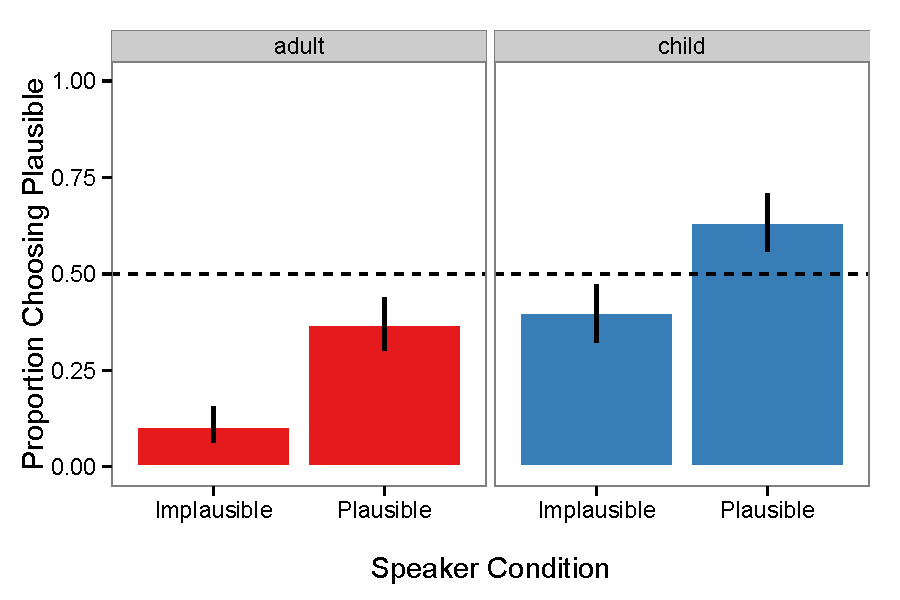
\includegraphics[width=\textwidth]{figures/exp1_results.pdf}
    \end{center}
    \caption{Experiment 1 test trial selections for both children and adults. In line with the predictions of a noisy channel model of language processing, both children and adults were more likely to correct the phonological error during test trials when they were previously exposed to a plausible speaker. Bars show group-averaged proportion of plausible item selection at test, error bars show 95\% confidence intervals computed by non-parametric bootstrap. The dotted line indicates chance perfromance.}%
   \label{fig:exp1_results}
\end{figure}

Did this exposure to a Plausible vs. Implausible speaker change participants' expectations during the ambiguous test trials? Figure~\ref{fig:exp1_results} shows the proportion of both children and adults who selected the plausible referent at test in both conditions. As predicted, both groups were sensitive to the manipulation, selecting the plausible referent more often in the Plausible Speaker condition. While children children were overall more likely to pick the plausible referent in both conditions, the size of the difference between conditions was comparable in adults and children, indicating equal sensitivity to the difference between speakers. To confirm these findings formally, we again fit a mixed effects regression predicting choice on test trials from group (child vs. adult), condition (Plausible vs. Implausible Speaker), and their interaction. Both of the main effects were significant, but the interaction was not, indicating that both children and adults  ($\beta_{child} = 1.96$,  $z = 3.33$, $p <.001$, $\beta_{Plausible Speaker} = 2.33$,  $z = 4.40$, $p <.001$,  $\beta_{child \: x \: condition} = -1.01$,  $z = -1.53$, $p = .13$).

When children and adults were exposed to a speaker who was likely to produce semantically implausible utterances (e.g. ``my cat has three little hammers''), the were more likely to interpret ambiguous utterances literally instead of error-correcting to a more semantically plausible alternative. Intriguingly, the size of this adaptation was comparable in both groups, suggesting that preschoolers are already adapting as rapidly and as adults. Children were, however, more likely overall to pick the plausible referent during ambiguous test trials, suggesting that they generally rely more on their expectations than do adults. This is consonant with other evidence showing significantly more noise in children's perceptual systems \cite{neuman1983}.

\section{Experiment 2}

Experiment 1 shows that children, to the same degree as adults, flexibly adapt their on-line language processing in accord with their expectations about what a speaker is likely to say. In Experiment 2, we replicate this finding and also test a further prediction of the noisy channel framework for language processing: listeners should adapt to the reliability of the acoustic signal. As speech becomes noisier, and thus harder to hear, listeners should rely more on their expectations. 

In addition, because all of the Test trials asked the listener to select the semantically implausible referent, it is possible that exposure to an Implausible speaker induced listeners to select the implausible referent at test generally, independent of their acoustic input.  In Experiment 2, we provide a control condition in which the Implausible speaker from training asked for the semantically plausible referent at test. If children inferred from the unambiguous Exposure trials that the goal of the game was to pick the ``silly'' referent, they should have continued to select the implausible referent on Test trials. In contrast, if Exposure trials caused them to adjust the relative weights on acoustic information and linguistic expectations, they should have selected the plausible referent at test.

\subsection{Method}

\subsubsection{Participants}

Children for Experiment 2 were recruited from the floor of the San Jose Children's Discovery museum. An experimenter approached the child and parent and obtained informed consent before inviting both to enter a separate room in which the iPad and camera were set up. Data was collected from a total of 114 children were collected, 1 of whom were excluded for insufficient exposure to English and 2 who were excluded for parent-reported developmental disabilities. As before, children were recruited until at least 20 had been run in each Condition. Children's ages and sexes were again comparable across conditions (Plausible, Noisy -- 26 children, 12 girls, age: mean = 4.98, min = 4.02, max = 5.94; Implausible, Noisy -- 24 children, 11 girls, age: mean = 5.01, max = 5.92, min = 4.01, Plausible, No Noise = 21 children, 8 girls, age: mean = 4.89, max = 5.93, min = 4.1, Implausible, No Noise --- 20 children, 12 girls, age: mean = 4.98, max = 5.83, min = 4, Control --- 20 children, 11 girls, age: mean = 4.96, max = 5,91, min = 4.15).
 
\subsubsection{Stimuli, Design, \& Procedure}

Stimuli were constructed as in Experiment 1 with a few small changes. First, one additional test trial was added to increase power. Second, two versions of each acoustic recording were made. One was recorded in a sound-proof room by a female native English speaker as before. The second was constructed by convolving each recording with randomly generated Brown noise with an amplitude of .7. The first was used in the No Noise conditions, the second was used to replicate the two conditions from Experiment 1 as well as for the Control condition.

\subsection{Results and Discussion}

As in Experiment 1, we first establish that children understood the task, and encoded the differences between the Plausible and Implausible speakers during Exposure trials. First, we ask whether participants selected the plausible referent when it was asked for by the Plausible speaker, and selected the implausible referent when it was asked for by the Implausible speaker independent of noise level. We submitted performance for each condition and noise level separately to a mixed-effects logistic regression with random effects of subject and trial. 

\begin{figure}[tb]
     \begin{center}
     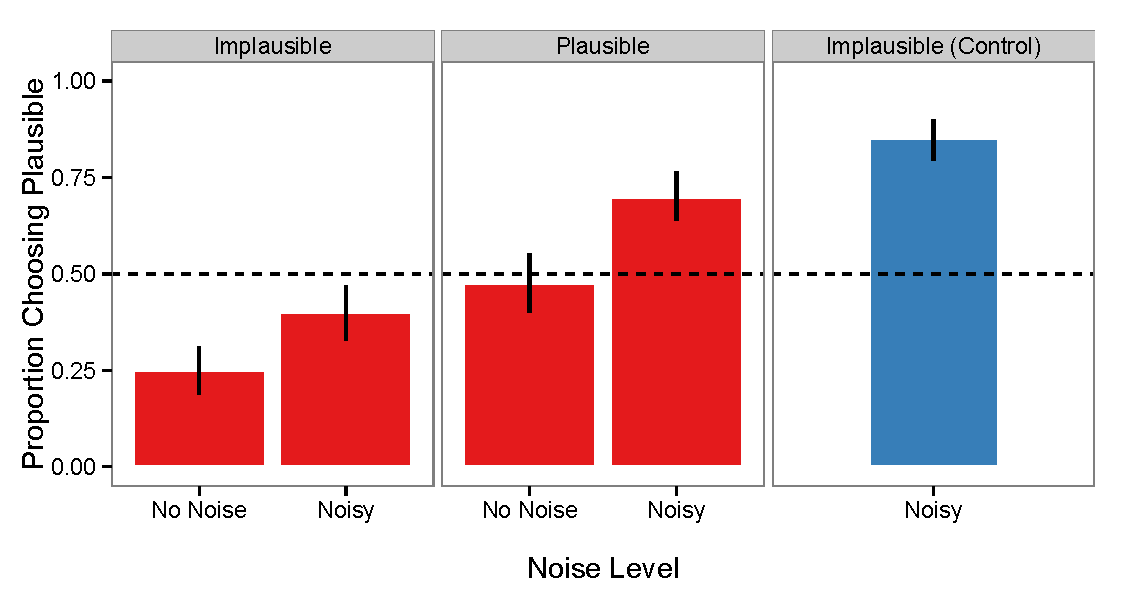
\includegraphics[width=\textwidth]{figures/exp2_results.pdf}
    \end{center}
    \caption{Experiment 2 results}%
   \label{fig:exp2_results}
\end{figure}


As before, children were more likely than chance to choose the plausible referent in the Plausible condition, but less likely than chance to choose the plausible referent when the speaker asked for the implausible referent (smallest $\beta_{Control} = -.153$, $z = -4.32$, p < .001). Second, we again compared the conditions to each other, fitting a mixed-effects regression predicting choice on Exposure trials noise condition (Implausible, Plausible, Control). Compared to the Implausible Speaker condition, children exposed to the Plausible Speaker were more likely to pick the Implausible referent on Exposure trials ($\beta_{Plausible} = 6.62$,  $z = 8.88$, $p <.001$). Children exposed to the Control speaker, who was identical to the Implausible speaker on Exposure trials, were not significantly different as predicted ($\beta_{Control} = .36$,  $z = .83$, $p = .42$). Further, the model showed a marginal effect of Noise level ($\beta_{Noisy} = .86$,  $z = 1.74$, $p = .08$) and a significant interaction between Noise level and Speaker ($\beta_{Plausible \: x \: Noisy} = -1.71$, $z= -2.15$, $p = .03$), indicating that the addition of noise moved children in both conditions closer to chance as expected.

Did children integrate noise level of the acoustic stimuli with Speaker expectations on the ambiguous test trials? Figure~\ref{fig:exp2_results} shows the proportion of both children and adults who selected the plausible referent at test in both conditions and under both noise conditions. As predicted, children showed sensitivity to both Speaker reliability and acoustic noise. Children selected the plausible referent at test, correcting the error in their acoustic input, more often when the Speaker had said plausible things on Exposure trials (as in Experiment 1). In addition, regardless of Speaker plausibility, children selected the plausible referent more frequently when the acoustic input was noisy. To confirm these findings formally, we again fit a mixed effects regression predicting choice on test trials from Speaker type and Noise level as well as their interaction. As predicted, both main effects were significant ($\beta_{1.20} = 1.96$,  $z = 3.20$, $p <.001$, $\beta_{Noisy} = .81$,  $z = 2.21$, $p = .03$), but their interaction was not ($\beta_{Plausible :\ x :\ Noisy} = .33$,  $z = .65$, $p = .51$).

Finally, we asked whether children who were responded to an Implausible speaker on Exposure trials always chose the implausible referent on test trials even when the speaker referred to the plausible referent. A mixed effects model estimating plausible referent on Test trials showed that compared to the Plausible speaker, children exposed to the Implausible speaker were less likely to pick the plausible referent ($\beta_{Implausible} = -1.57$,  $z = -4.14$, $p <.001$), but children in the control condition were \emph{more} likely to select the plausible referent ($\beta_{Control} = 1.06$,  $z = 2.05$, $p = .04$). Thus, children who were asked for the plausible referent at test selected it, even when the speaker had previously always referred to the implausible referent. This is further evidence that children were attending to and responding to the acoustic input from the speaker on Test trials and not just relying on expectations.


\section{General Discussion}

Summarize what we did

Adults vs. kids - perceptual certainty. And this finding makes predictions about atypical development. Worse language models for kids, or less perceptual certainty. 

We see here a tradeoff between two models, perception and expectation. But what is the substance of these models? Challenge for future work. Is it pragmatics all the way down? Or are these lower level models based on perceptual similarity and word-coccurrence?

How to integrate with failures of pragmatics and ambiguity resolution? Our paradigm here is lexical and grounded and children have lots of experience with it. Failures tend to happen in cases where complex syntax or abstract semantics (e.g. quantifiers) are at issue - in these cases, more experience is necessary to have a good predictive model, even if you can do some comprehension. 

The end!

\section{Acknowledgments}

We are grateful to Nicolette Castro for collecting the bulk of the child data, and all of the members of the Language and Cognition Lab for their feedback on this project. In addition, we thank the parents, children, and staff at the San Jose Children's Discovery Museum for supporting us in collecting developmental data. This work was supported by NIH NRSA F32HD075577 to DY as well as grants from the Merck Scholars Foundation and the Stanford Center Health Research Initiative to MCF.

\bibliographystyle{apacite}
\bibliography{noisy_kids}

\end{document}
